\subsection{Background: DMA Datapath in Virtualized Environments}
\label{vfree:sec:background-datapath}
This section gives an overview of the DMA datapath 
    in virtualized environments with strict IO memory protection.
% Figure ~\ref{vfree:fig:datapath}  illustrates the NIC-to-memory datapath 
%     when memory protection is enabled in a virtualized environment.
% We base our discussion on the datapaths of CX-7 Mellanox NICs with Intel CPUs; 
% the high-level datapath for other NICs and CPUs is similar \todo{citation}.
% the guest OS 
%    maintains the mappings from each IO Virtual Address (IOVA)
%    to its corresponding Guest Physical Address (GPA)
%    in the guest I/O page table (IOPT);
%    the host OS maintains the mapping from 
%    each GPA to the Host Physical Address (HPA) 
%    in the host IOPT. 
% A DMA requires a {\it nested translation} from 
%    IOVA to GPA and then from GPA to HPA;
%
% \rachit{
% High-level notes:
% \begin{itemize}
    % \item use ``guest'' rather than ``guest NIC driver'' unless that distinction is super important
    % \item mention that we primarily focus on strict safety mode
    % \item too many acronyms may confuse people (eg, Tx, TCP, ACKs, IOMMU, NIC, DMA, API, vIOMMU, IO, IOVA, GPA, HPA, IOTLB, IOPT, PCIe in the next two paragraphs): try to minimize; also find a way to make it easier: maybe use {\tt iova} rather than IOVA?
% \end{itemize}
% }
%
% We discuss the DMA datapath in virtualized environments. 
Throughout the paper, we consider device passthrough which grants the guest direct access 
    to the physical NIC---the guest can directly post IO descriptors to the NIC without host intervention. 
For brevity, we focus on the Linux network stack, Intel Emerald Rapids CPUs, and Nvidia CX-7 NICs. 
% We keep the discussion focused on 
%    {\it strict} IO memory protection~\cite{Amit2011vIOMMU,Rubin2024FastSafe}.

% \schai{To achieve close-to-native I/O performance, we utilize device passthrough to grant the guest OS direct access to the physical NIC. 
% This allows the guest OS can directly program the NIC through MMIO registers;
% for example, it can post I/O descriptors to NIC without any hypervisor intervention. }

% ---and intra-guest protection\saksham{we need to concretely define and motivate why we care about intra-guest protection somewhere}. 

IO memory protection is realized by providing NICs with IO virtual addresses (IOVAs).
%     to DMA data. 
To execute a data transfer, the host hardware translates IOVAs to corresponding physical addresses 
    using an IOMMU and an IO page table (IOPT) that stores IOVA-to-physical address mappings. 
    The translation is sped up using hardware caches, including 
    an IOTLB and IOPWCs for the final 
    and intermediate translations~\cite{Rubin2024FastSafe}. 

Figure~\ref{vfree:fig:datapath} illustrates the lifetime of a DMA operation under IO memory protection, 
    breaking down the datapath in three phases: 
    (1) Pre-DMA phase, involving creation of address mappings and supplying IOVAs to NIC; 
    (2) DMA phase, involving performing address translation and DMA transfer; 
    and (3) Post-DMA phase, involving destruction of address mappings 
    and invalidating address translation caches in hardware. We describe these three phases in detail below. 

\begin{figure}[H]
	\centering
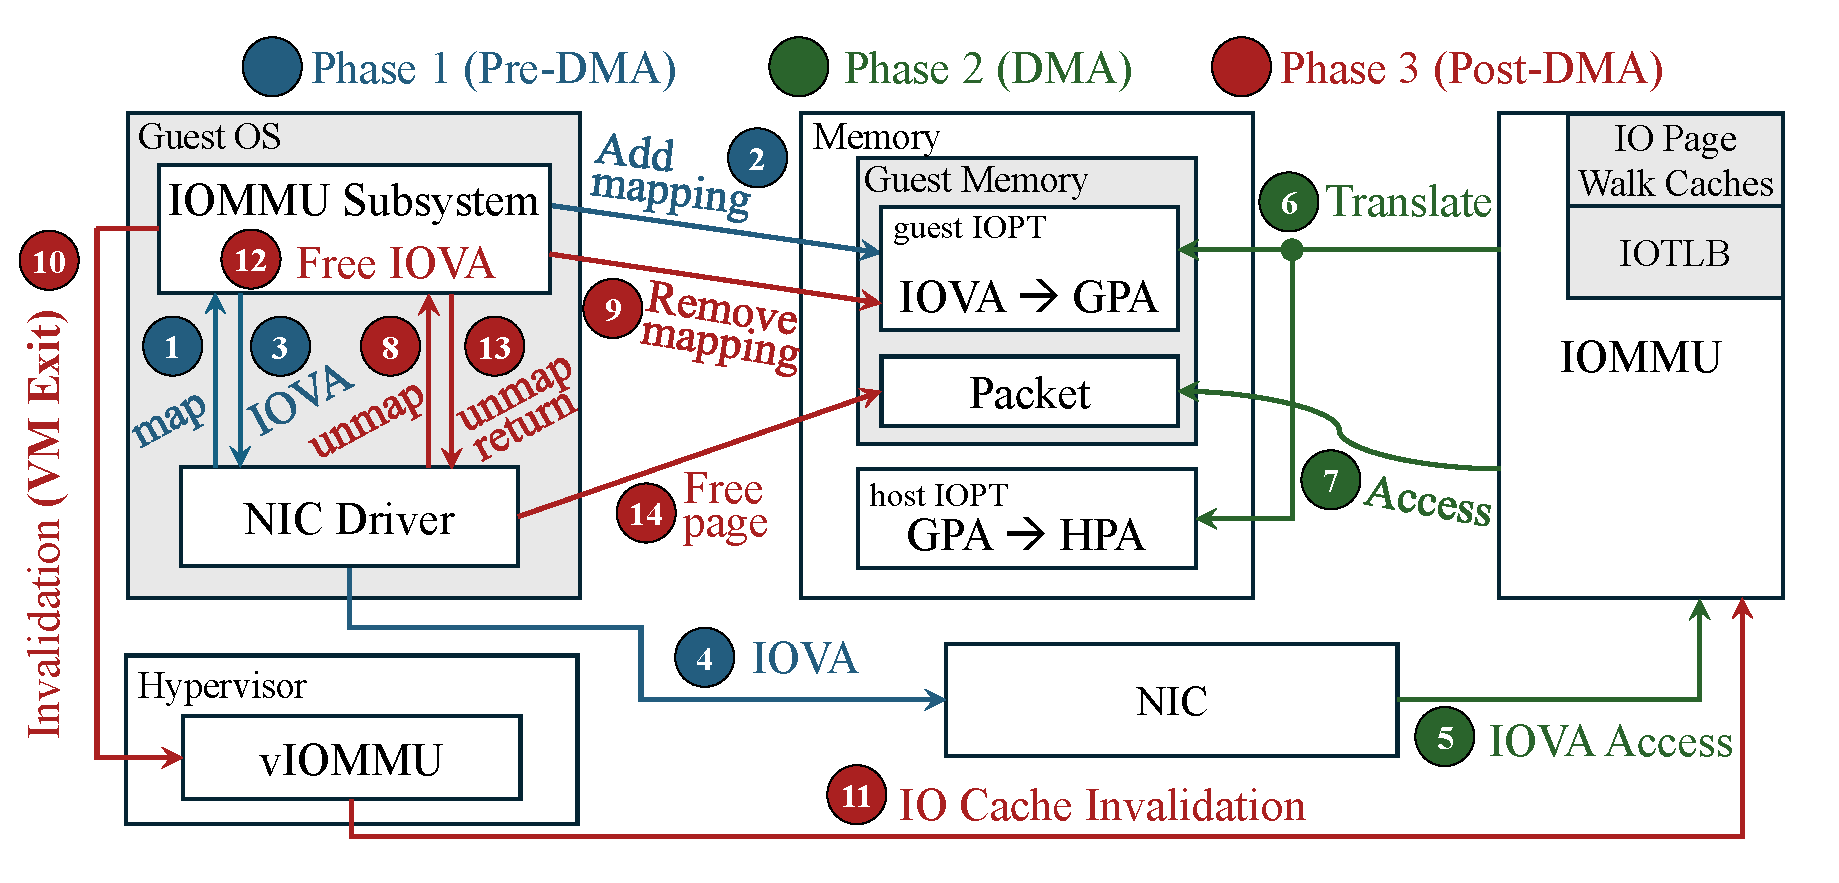
\includegraphics[width=\columnwidth]{figures/datapath_large_font_cropped.pdf}
\Description{ Illustration of NIC-to-memory DMA datapath at the transmitter when memory protection is enabled.}
\caption{\small {\bf Illustration of NIC-to-memory DMA datapath at the transmitter when memory protection is enabled.}}
\label{vfree:fig:datapath}
\end{figure}

% Bypassing the hypervisor on the I/O data path is essential to saturate modern high-speed networks bandwidth. 

% Crucially, while this passthrough mechanism applies to the NIC, it does \emph{not} extend to the host's IOMMU. 
% The IOMMU remains a shared hardware resource managed by the host, and current architectures preclude VMs from directly manipulating its hardware registers~\cite{intel_vtd_spec,qemu_10_0}.
% Consequently, the Post-DMA phase—which involve invalidating IOMMU state—still necessitates hypervisor intervention, as detailed below.
% }\saksham{I think we can get rid of this para.}

% We use Intel Emerald Rapids CPUs and Nvidia CX-7 NICs; the high-level datapath for other recent CPU architectures and NICs is similar. 

% Further, we also assume device passthrough/direct device assignment\saksham{say why?}. 

% assumptions: intel CPUs, device passthrough, linux, nested translation in IOMMU, intra-guest, viommmu in QEMU, focus on strict


\para{\BC{1} IOVA allocation and IOMMU mapping.} 
% Before the NIC is allowed to DMA the data to/from the host memory, 
The guest uses the \CodeIn{map()} API to create an IOVA-to-GPA (guest physical address) 
    mapping in the guest-local IOPT. 
The guest then creates a packet descriptor containing the IOVA, and passes 
    the descriptor to the NIC.
% \footnote{There's a slight difference in exactly when the packet descriptors (hence IOVA mappings) are created and communicated to the NIC between the NIC transmit (Tx) and receive (Rx) datapath. For Tx, descriptors are created whenever the application has some data ready to be sent to the socket, while for Rx the descriptors are pro-actively filled-up to handle future packet arrivals at the NIC. \saksham{Folks should check this footnote, and make it slightly more precise.}}. 

With device passthrough, the NIC performs data transfers without involving the host. This is possible with IOMMUs in recent Intel CPU architectures (Sapphire Rapids and newer) using 
    nested translation~\cite{intel_vtd_spec} that enables the  
    IOMMU to translate IOVAs directly to corresponding host physical addresses (HPAs) rather than GPAs,
    without host intervention.\footnote{We focus on nested translation supported by modern server hardware. 
    An alternative is to {\it shadow IOPT}, where the hypervisor 
    maintains an IOPT that maps each IOVA directly to the HPA.
    Shadow IOPT requires every new mapping to trigger a VM exit 
    for the hypervisor to update the shadow IOPT. Nested translation eliminates such VM exits.
    In our measurement, nested translation achieves strictly higher throughput than shadow IOPT,
    by 1.2$\times$ to 2.6$\times$ across core counts. 
    While we focus on nested translations, some of our techniques may also be useful for shadow IOPT.} 

\if 0
With nested translation, IOMMUs support two levels of address translations: 
    IOVA-to-GPA translation using per-guest IOPT, along with GPA-to-HPA translation 
    using a host-based IOPT. 
Typically, GPA-to-HPA updates happen infrequently (e.g., when creating a new VM), 
    and hence not on the critical path of NIC DMA operations. \rachit{why do we need this paragraph; the previous paragraph already says that nested translation enables iova-to-hpa translation}
%in this paper, we assume GPA-to-HPA mappings remain static. \leshna{I do not like this framing here, this seems like we assume the mapping to remain static only for our approach, whereas that is how it is handled in QEMU, basically a supporting statement of why this assumption is not very huge}
\fi


% To prepare a packet for transmission, the guest    invokes the DMA mapping API to map the memory page containing the packet data.
% The vIOMMU subsystem assigns an I/O virtual address (IOVA) and 
%     installs a mapping from the IOVA to the corresponding Guest Physical Address (GPA) 
%     in the guest I/O page table (IOPT);
%     the IOVA is then returned to the NIC driver.

    
% Upon DMA, the GPA is further translated by the host into a Host Physical Address (HPA).
% The host establishes the GPA-to-HPA mappings when allocating memory to the VM. 
% These mappings change infrequently and are not on the critical path of DMA operations. 
% In contrast, the guest dynamically installs IOVA-to-GPA mappings 
%     for DMA buffers. 
% When a new IOVA-to-GPA mapping is created, no host intervention or IOTLB invalidation 
%     is required because the IOVA can only be reused after the device has no stale cache translations.
   
% As a result, the mapping operation proceeds entirely within the guest without triggering a VM exit.

%        The hypervisor intercepts this invalidation,\rachit{allocates a physical page at this point?} updates the shadow page table, 
% and issues the hardware invalidation on the guest's behalf. 
% Thus, under shadow page tables, every new IOMMU mapping requires a VM exit in addition to the unmap-path VM exit. 
% We present comparative results for shadow and nested translation in \todo{fig}}

% \footnote{Under shadow page tables, the hypervisor maintains a single merged IO page table mapping IOVAs directly to HPAs.
% Because the hypervisor has no other mechanism to learn about new guest mappings, the guest must issue an IOTLB invalidation after every new mapping ---- a privileged operation that triggers a VM exit. The hypervisor intercepts this invalidation,\rachit{allocates a physical page at this point?} updates the shadow page table, and issues the hardware invalidation on the guest's behalf. Thus, under shadow page tables, every new IOMMU mapping requires a VM exit in addition to the unmap-path VM exit. We present comparative results for shadow and nested translation in \todo{fig}}

\if 0
% discussed with Leshna and this is not super relevant
\question{we have a lot of ways this is handled, do we want a description? Do I say we focus on static pinning as that will give us the best performance?, 
    On-demand page pinning (original vIOMMU paper) — hypervisor creates GPA to HPA mappings lazily, 
    invalidations; IOMMU hardware page faults (PRI/PRQ) 
    — the IOMMU itself can fault on a missing second-stage entry 
    and the hypervisor populates it on demand, 
    Dynamic scenarios like memory ballooning, live migration, etc. 
    that mutate second-stage mappings at runtime or static pinning we see in our case}
\fi

 % To initiate DMA, the guest writes the IOVA of the packet buffer 
    % into a Tx descriptor and notifies the NIC.
    % \rachit{\circled{4} should be a part of step \circled{2} in the figure?}


 \para{\BC{2} DMA and address translation.} 
The NIC issues DMA requests using the IOVA in packet descriptors,
    which triggers IOVA-to-HPA address translation using the IOMMU; 
% \leshna{this reads to me like the NIC and IOMMU are tightly coupled, like the IOMMU is part of the NIC} 
the final or intermediate translation 
    could be cached in IOMMU's IOTLB and IO PWCs~\cite{Rubin2024FastSafe}. Upon successful translation, the DMA is executed to the corresponding HPA. 
% to fetch the packet data from host memory 
    % before transmitting it over the network. 
% A single DMA operation may be split into multiple PCIe transactions 
%     depending on the request size and the maximum PCIe transaction size supported by the device and the platform.

% As these PCIe transactions reach the root complex (e.g., the Integrated I/O Controller in Intel architectures), 
%     the IOVA in each transaction must be translated into a HPA. 
% The IOMMU first consults its IOTLB. 
% On an IOTLB hit, the cached translation is used to obtain the corresponding HPA. 
% On a miss, the IOMMU performs a IOPT walk to resolve the translation, 
%     potentially involving nested translation across the guest and host IOPTs. 
% As address translation occurs at the granularity of individual PCIe transactions, 
    % multiple translations may be required to complete the DMA transfer for a single packet.
% \rachit{This paragraph should be significantly cut down; information that seem important to the rest of the paper: to initiate DMA, the guest informs the NIC of the iova; the NIC performs address translation using IOMMU; gets a physical address and transmits data at that physical address (there should be a data copy involved somewhere). requires no VM exits.}

% both stages; paging-structure caches may accelerate this walk 
%    by caching intermediate entries from either or both stages. 
\if 0
\rachit{would be nice to say how to this about nested page tables in terms of levels 
    (e.g., can L1 cache store the first level of first-stage AND the first level of second-stage?)}
\leshna{
    This in the spec explicitly mentions everything is allowed,
   the can combine or do one, based on hardware}. 
\fi

\para{\BC{3} Completion and IOMMU cache invalidation.} 
To maintain strict IO memory protection, NIC's access to the target page(s) in the host memory must be revoked immediately after the DMA completes~\cite{Rubin2024FastSafe,Amit2011vIOMMU}. This happens using two steps.
% \rachit{explicitly say: To do so, the guest invokes unmap() call which leads to removal of ....}
First, the guest uses the \CodeIn{unmap()} API which removes 
    the corresponding IOVA-to-GPA mapping from the guest IOPT.\footnote{GPA-to-HPA mapping are managed by the host. In KVM/QEMU, these mappings are established at VM creation time; for VFIO passthrough devices, guest memory is pinned, so GPA-to-HPA mappings remain static.} % and are not on the DMA critical path.} %This paper focuses on the IOVA-to-GPA mappings that 
    % change with every \CodeIn{map}/\CodeIn{unmap}.}} 
Second,
    mappings in IOMMU caches are also invalidated---typically, these invalidations are executed synchronously within the \CodeIn{unmap()} call.
The IOMMU provides an invalidation queue as an interface for the OS 
    to submit {\it invalidation requests (IRs)}. This happens in two steps (see Figure~\ref{vfree:fig:ir-ops}). 


   

\begin{enumerate}
\item {\bf Preparing the IR descriptor (IR-PREP).} 
% The first step is preparing an IR to submit to % processed by the IOMMU hardware. 
The guest kernel thread first acquires 
    a per-IO-domain 
    spinlock (termed \CodeIn{cache\_lock}~\cite{dmar_domain.cache_lock} in Linux). 
    Upon acquiring the lock, the thread prepares and enqueues 
    an IR descriptor in a per-IO-domain submission queue---referred 
    to as {\it IO-domain queue} in the guest. 
Note that there can be multiple IO-domain queues in the guest
    (\textit{e.g.}, for different devices).
%    \rachit{this may confuse the reader: if the thread keeps both cache-lock and q-lock, why does it need to copy the request to the SW queue; why can't it directly write to the emulated invalidation queue?}

% \rachit{IIRC, we never define a device, and never say that devices share IO virtual address spaces; we should define devices and say it in S2}. \rachit{is it true that only the vCPUs within a single VM contend on this lock? are vCPUs in different VMs in different domains in vIOMMU?}
% As an IOMMU domain may have multiple physical devices, the kernel needs to ensure the IOMMU caches for each of the devices are flushed. 
% While holding this lock, the thread iterates over the domain's list of \emph{cache tags}---metadata 
%     entries that record which hardware caches may hold translations for IO devices in this domain (e.g., IOTLB in IOMMU or ATS-supported NICs~\cite{}\saksham{need references}). 
% For each cache tag, the kernel prepares the appropriate IR, specifying the IOVA range to invalidate. 
% % and whether to flush IOTLB entries alone or additionally flush page-table cache entries. The descriptors are accumulated into a batch for the physical IOMMU hardware unit of the device. 
% % \rachit{the text is very clear now, great. However, I (and hence, may be other readers) wonder: why does the kernel need to ensure that IOMMU caches for all devices are flushed? [Update] Ha, I see it is answered in the next paragraph.}.
% The lock ensures safe access of the cache tags for IR-PREP,
%     preventing data races caused by concurrent updates 
%     of the cache-tag list (e.g., a concurrent 
%     detach of an I/O device would free its cache-tag list).
% % Specifically, if a device were detached while iterating over the list, the cache tag entry could be freed underneath the iterator, resulting in a use-after-free.  
% % Conversely, if a device were attached mid-flush, the new device's caches might not receive the invalidation, leaving stale translations that violate the strict guarantee.  \CodeIn{cache\_lock} serializes flushes against structural
% % modifications to prevent both hazards.
% % \rachit{use-after-free discussion makes sense but this is a cache, so use-after-free should not lead to any errors---right?}
% % For the device attachment, why would a newly attached device have cache entries?}
% However, this lock serializes IR-PREP operations 
%     for all threads in the same IO domain in the VM.
% Upon acquiring the lock and preparing the IR, it is enqueued in a (per-IO-domain) submission queue---referred 
%     to as SW queue within the guest kernel\saksham{check if true}.

\item {\bf Submitting the IR to IOMMU hardware (IR-SUB):} 
% \para{\circledx{2} Hardware queue submission under \CodeIn{q\_lock}.} 
To submit the IR descriptors in an IO-domain 
    queue to the IOMMU hardware, 
    the hypervisor, specifically the vIOMMU subsystem, exposes 
    an {\it emulated IOMMU invalidation queue} to the guest.
% This is the interface available to each guest to submit IRs to the IOMMU hardware. 
Before submitting the IR to the emulated invalidation queue, the guest needs to acquire another lock---a 
    per-invalidation-queue spinlock (\CodeIn{q\_lock}{~\cite{q_inval.q_lock}} in Linux). 
% This serializes access to the emulated invalidation queue for IRs from all threads within the guest; 
% otherwise, concurrent writers could corrupt the queue by overwriting each other's IRs. 
    While holding \CodeIn{q\_lock}, the kernel writes the IR descriptor into the queue, 
    then advances a tail register---via an MMIO write---to signal the hardware 
    to process the IR. 
% \rachit{guest/kernel inconsistency; also the text says that the ``the'' guest thread: is it different from the network thread above?}
\end{enumerate}






 % While holding \texttt{q\_lock}, the kernel writes the batch of invalidation descriptors and a trailing wait descriptor into the queue, then advances the tail register via an MMIO write.

    % \para{\circledx{3} VM~exit and busy-wait.} 
    %  The MMIO write to the tail register triggers an \texttt{EPT\_MISCONFIG} VM~exit, transferring control to the hypervisor.  The hypervisor validates the invalidation request, issues the corresponding hardware invalidation on the physical IOMMU, and returns control to the guest.  The guest CPU then busy-waits on the status field written by the wait descriptor until the hardware signals that the invalidation is complete.  Only then are both locks released and the physical page made available for recycling.
\noindent
{\bf Unavoidable VM exit for {\em every} IR.} 
Submitting IRs from the guest to the IOMMU hardware necessarily requires hypervisor intervention. 
This is because the IOMMU invalidation queue---the interface provided to the OS for IOMMU cache invalidation---is 
    a shared host resource with no per-VM partitioning~\cite{intel_vtd_spec_caching}; 
    allowing multiple guests to write concurrently would risk corruption. Thus, the MMIO write to the tail register
% Every IR-SUB operation to the emulated invalidation queue 
triggers a 
% \CodeIn{EPT\_MISCONFIG} 
VM~exit, transferring control to the hypervisor.  The hypervisor validates the IR, issues the corresponding IR to the physical IOMMU (by copying the IR to the IOMMU invalidation queue in the host), and returns control to the guest.  The guest thread, in the meantime, busy-waits on the status field until the hardware signals that the invalidation is complete.  
% Consequently, the guest must trap into the host, incuring an unavoidable VM exit~\cite{qemu_intel_iommu_c} during unmaps.
% Only then are both locks released.
So, the VM exit is performed for {\em every} IR,
because an IR descriptor is written to the emulated queue protected
    by \CodeIn{cache\_lock} (\CodeIn{q\_lock} 
    is acquired \emph{inside} \CodeIn{cache\_lock}). 
% The nesting of the two critical sections is not a major performance bottleneck
    % on bare mental (taking less than one microsecond).
% However, it becomes significantly more expensive in virtualized environment (see \S\ref{vfree:sec:pointer}).
% This is likely done to avoid re-acquiring the \CodeIn{cache\_lock} 
%    to copy the IR from the SW queue to emulated invalidation queue \rachit{I understand we are doing it in our final design (as we discussed)? if so, we should avoid this sentence otherwise we need to outline our key insight on why we can do it.}. 
% Therefore, each IR triggers an independent VM exit. 

 





% Each physical IOMMU has its own invalidation queue



 % and its own \CodeIn{q\_lock}; 

    
% This queue is shared across all cores; 
% While holding \CodeIn{q\_lock}, the kernel writes the batch of invalidation descriptors and a trailing wait descriptor into the queue, then advances the tail register via an MMIO write.





% \rachit{a bit of restructuring the rest of this paragraph will be helpful: while the guest can remove iova-to-gpa mappings, mappings in IOTLB and IOPT caches must also be invalidated---this requires hypervisor intervention; then move the next two sentences to after describing why the intervention is needed.}

\begin{figure}[H]
	\centering
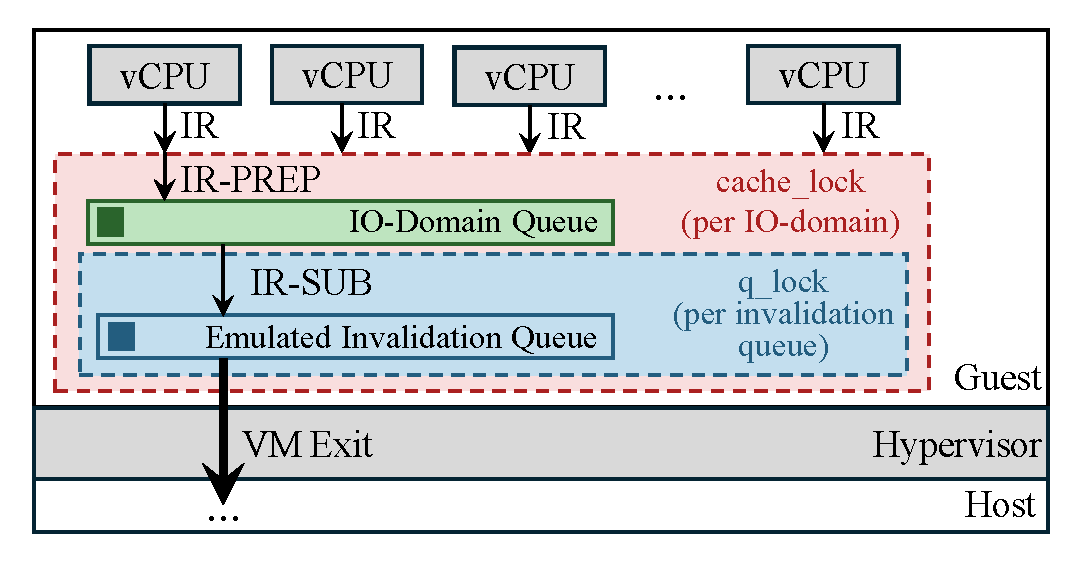
\includegraphics[width=0.72\columnwidth]
{figures/background_guest_queues_cropped.pdf}
\caption{\small {\bf IR-PREP and IR-SUB operations in the Post-DMA phase and the corresponding queues.}}
\label{vfree:fig:ir-ops}
\end{figure}

% The vIOMMU then invalidates the affected entries in all IOMMU caches, including the IOTLB and IOPT caches, 
    
    
% \saksham{Need to describe the invalidation process in more details here, the cache lock, shared SW Q, q lock, emulated HW q, hypervisor trap, and corresponding host operations.} \saksham{Also talk about strict safety guarantee here, about synchronously invalidating after unmaps.}


% Unlike mapping new pages, unmapping \emph{always} 

% , which serializes invalidation requests 
%     and issues the hardware invalidation on the guest's behalf. 
    
 % \para{\circledx{3} VM~exit and busy-wait.} 

\noindent
Finally, upon successful IR processing, the IOVA is returned to the IOVA allocator and the corresponding physical page(s) 
    used for DMA are made available for recycling. 
Both \CodeIn{cache\_lock} and \CodeIn{q\_lock} are released when IR-SUB finishes.
% \rachit{say when the locks are released}

% \vspace{0.1in}
% \paragraphb{Strict memory protection} Linux today enforces strict memory protection by performing IR processing synchronously with {\tt unmap()} call. 

% \paragraph{Tx Datapath}
% \label{vfree:sec:tx-datapath}
% Every transmitted network packet---including TCP \leshnaedit{acknowledgements} generated in response to received data---goes
%     through a per-packet IOMMU lifecycle in the follows steps:
% %\begin{enumerate}[leftmargin=*,label=\protect\circledb{\arabic*}]
% % \item 
% \paragraph{\bf Rx Datapath.}
% \label{vfree:sec:rx-datapath}
% The Rx datapath follows the IOMMU mapping, address translation, and invalidation steps (\BC{1}--\BC{3}) as the Tx datapath steps, 
%     but does so in the reverse direction: the NIC DMAs incoming packet data 
%     into host memory rather than reading it out. 

\para{Optimizations for Rx Datapath in Linux.}
% \label{vfree:sec:linux-opt}
Recent versions of Linux network stack (>=6.11~\cite{linux_page_pool_netmem}) implement
    an optimization in the Rx datapath to reduce \CodeIn{map()}
    and \CodeIn{unmap()} operations.{\footnote{For several pragmatic reasons, existing operating systems do not apply similar optimizations on the Tx datapath.
% , 
%     because typically no data-copy operation is involved between the kernel and userspace buffers: 
%     NIC directly DMA's data from the userspace \rachit{are we sure?} buffers in the Tx datapath, 
%     and the NIC can maliciously access the DMA buffers if permanently mapped IOVAs are used. 
%
Hence, every transmitted packet incurs at least one VM exit per \CodeIn{unmap()} call.}}
It uses a per-CPU cache to maintain a set of IOVAs permanently mapped to the IOMMU~\cite{markuze2018damn}. 
In the Rx datapath, the kernel uses the physical pages mapped to these IOVAs to allocated kernel-space buffers 
    (\textit{e.g.}, TCP socket buffers), used to DMA data from the NIC. 
Upon DMA, the data is copied from kernel-space buffers to the userspace buffers, 
    before returning back the IOVA to the cache.
Malicious NIC with access to the IOVA cannot access the userspace buffers (which are not mapped to the IOMMU). 
Using (and recycling) these IOVAs therefore do not require \CodeIn{map()}/\CodeIn{unmap()} calls. 
This optimization is helpful for workloads for which actively used IOVAs are consistently smaller than the cache size~\cite{Rubin2024FastSafe}. 
Upon exhausting this cache, whenever the kernel requires another IOVA, 
it uses the default IOVA allocation/deallocation datapath, 
using regular \CodeIn{map()}/\CodeIn{unmap()} operations.
%  as discussed previously in this section.
% The page pool consists of a small per-CPU cache (64~entries in mlx5 \tianyin{??}) backed by a larger pointer ring (1024~entries) \rachit{is it important to distinguish between the two? if not, that seems unnecessary detail}. 
% Every page in the pool carries a valid IOVA mapping, established when the page first enters the pool and persists as long as the page remains in it. 
% On the receive fast path, the driver retrieves a pre-mapped page from the cache, installs its IOVA into an Rx descriptor, and marks it ready to receive---no IOMMU interaction is needed. Upon completion of DMA, the page is returned to the page pool. If the pool has space (the cache or pointer ring is not full), the page is placed back with its IOVA mapping unchanged. No IOMMU operation occurs and no VM~exit is triggered. 



% {Why it works for Rx side only?}
% This is feasible because on the receive side, the driver owns the page from allocation through free and can keep it persistently mapped without friction. 
% On the transmit side, no such pool exists because the kernel does not often own the page being sent. the payload resides in userspace memory; thus, the driver cannot recycle the userspace pages in a pre-mapped pool without performing expensive data copies. 


% An important difference is that modern NIC drivers maintain a per-CPU \emph{page pool} that eliminates most IOMMU operations from the Rx fast path. 

% \leshnaedit{In our setup \S\ref{vfree:sec:inefficiencies}, over 99.9\% IOMMU operations on the Rx data path are skipped by page pool.}







